\documentclass{beamer}

\mode<presentation>
{
	\usetheme{Boadilla}
	\beamertemplatenavigationsymbolsempty
	\setbeamercovered{transparent}
}
\usepackage[english]{babel}
\usepackage{color}
\usepackage{booktabs}
\addto\captionsenglish{\renewcommand{\figurename}{Source}}
\setbeamerfont{caption}{size=\scriptsize}

\newcommand\blfootnote[1]{%
	\begingroup
	\renewcommand\thefootnote{}\footnote{#1}%
	\addtocounter{footnote}{-1}%
	\endgroup
}

\title[Financial prediction with Neural Networks]{{\footnotesize Bachelor's Thesis} \vspace{1ex} \\ Financial prediction with Neural Networks}
\subtitle{``Predicting Spread Prices on VIX Futures with Deep Learning''}
\author[Thomas Leyh]{by Thomas Leyh}
\institute[]{University of Freiburg \\
			 Department of Computer Science \\
		 	 Computer Vision Group \\
		     Prof. Dr. Thomas Brox}
\date{September 12th, 2017}

\begin{document}

\frame{\titlepage}
\begin{frame}{Outline}
	\tableofcontents
\end{frame}

\AtBeginSection[]
{
	\begin{frame}<beamer>{Outline}
	\tableofcontents[currentsection]
	\end{frame}
}

\section{Why do this?}
\subsection{Some financial terminology}
\begin{frame}{Some financial terminology}
	\begin{columns}
		\begin{column}{0.65\linewidth}
			\begin{description}[<+(1)->]
				\item[VIX] \emph{CBOE's Volatility Index} based on the \emph{S\&P 500 Index} \\ (similar to the German \emph{DAX}).
				\item[Volatility] Measures the risk of sharp market movements.
				\item[Futures] A standardized tradable contract. The holder is guaranteed the delivery of the underlying commodity at its expiration.
				\item[Term structure] Formed by multiple futures with different expirations.
			\end{description}
		\end{column}
		\begin{column}{0.25\linewidth}
			\visible<4->{%
			\begin{figure}
				\includegraphics[width=1\linewidth]{images/potatoes}
				\caption{Jean Weber, INRA (Wikimedia Commons)}
			\end{figure}}
		\end{column}
	\end{columns}
	
\end{frame}

\subsection{The actual problem}
\begin{frame}{The actual problem}	
	\begin{columns}
		\begin{column}{0.5\linewidth}
			We are interested in the \alert{correction} of the term structure:
			\begin{itemize}
				\item Will it get corrected? \\
				{\small Do we invest in the first place?}
				\item At what position? \\
				{\small Where to place the spread?}
				\item When will the correction occur? \\
				{\small How long to hold the spread?}
			\end{itemize}
		\end{column}
		\begin{column}{0.5\linewidth}
			\centering
			\includegraphics[width=0.85\linewidth]{images/termstructure_sep} \\
			\hspace{4ex} \includegraphics[width=0.4cm]{images/arrow_down_red} \hspace{1ex} {\Huge \textbf{\alert{?}}} \\
			\includegraphics[width=0.85\linewidth]{images/termstructure_sep_corr}
		\end{column}
	\end{columns}
\end{frame}

\subsection{Where machine learning comes in}
\begin{frame}{Where machine learning comes in}
\begin{columns}
	\begin{column}{0.65\linewidth}
		We want some working model for this prediction. \\
		But we are too lazy to build it ourselves. \\
		$\rightarrow$ Let the computer do it.
		\\
		\begin{enumerate}
			\item Select appropriate model family
			\item Optimize hyperparameters
			\item Throw data at it
			\item \dots
			\item Profit
		\end{enumerate}
	\end{column}
	\begin{column}{0.3\linewidth}
		\centering
		This day's futures \\
		$\downarrow$ \\
		\fbox{Machine Learning} \\
		$\downarrow$ \\
		Next day's spreads
	\end{column}
\end{columns}
\end{frame}
\begin{frame}{Where machine learning comes in: Neural Networks}
	\begin{figure}
		\begin{columns}
			\begin{column}{.6\linewidth}
				\centering
				\includegraphics[width=\linewidth]{images/MultiLayerNeuralNetworkBigger_english}
			\end{column}
			\begin{column}{.2\linewidth}
				\caption{Chrislb (Wikimedia Commons)}
			\end{column}
		\end{columns}
	\end{figure}
	\vspace{-10pt}
	Equivalent to:
	\begin{align}
		&f^{(1)} \left(
		\underset{\text{inputs}}{
		\begin{bmatrix}
		y^{(0)}_1 \\ y^{(0)}_2 \\ y^{(0)}_3
		\end{bmatrix}}^\top \cdot
		\underset{weights}{\begin{bmatrix}
		w^{(1)}_{1,1} & w^{(1)}_{1,2} & w^{(1)}_{1,3} \\
		w^{(1)}_{2,1} & w^{(1)}_{2,2} & w^{(1)}_{2,3} \\
		w^{(1)}_{3,1} & w^{(1)}_{3,2} & w^{(1)}_{3,3}
		\end{bmatrix}}
		\right) &&= 
		\underset{\text{hidden layer}}{y^{(1)\top}}
		\\
		&f^{(2)} \left( y^{(1)\top}W^{(2)} \right) &&= 
		\underset{\text{outputs}}{y^{(2)\top}}
	\end{align}
	with often very simple \alert{activation function $f$} working elementwise.
\end{frame}

\section{Approaches}
\subsection{Data representation}
\begin{frame}{Data representation}
	\begin{itemize}
		\item<1-> There were \alert{2656 samples} used
			\begin{itemize}
				\item From October 23th, 2006 to May 11th, 2017
				\item Split with ratio 70:15:15 for training, validation and testing
				\item Optionally using minutely data
			\end{itemize}
		\item<2-> Preprocessing of the \alert{input data} -- today's futures --
			\begin{itemize}
				\item The difference between the term structures' legs was used
				\item A combination of additional inputs was used, \\ mostly \emph{days until expiration}
				\item Optionally centered and normalized
			\end{itemize}
		\item<3-> Choosing the \alert{target data} -- tomorrow's spreads --
			\begin{itemize}
				\item Predict all spreads at once \\
				or
				\item Predict one spread at a time \\
				or
				\item Just predict if prices will fall, rise or stay the same
			\end{itemize}
	\end{itemize}
\end{frame}

\subsection{Network architecture}
\begin{frame}{Network architecture}
	\alt<2>{
	\begin{figure}
		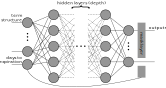
\includegraphics[width=\linewidth]{images/architecture1}
	\end{figure}
	}{Using \alert{Feedforward Neural Networks}. \\
	A very basic model where layers are simply stacked on top of each other.
	\vskip1em
	Hyperparameters:
	\begin{description}
		\item[Depth] Number of hidden layers
		\item[Width] Number of nodes per layer
		\item[Activations] For introducing nonlinearity at each at each node's ouput
		\item[Loss function] For comparing predictions and target values at the network's end (here: \emph{mean squared error})
		\item[Optimizer] For iteratively updating the weights (mostly \emph{Adam})
		\item[Regularizations] So the network doesn't just learn data by heart
		\item[\dots] and many more \dots
	\end{description}}
\end{frame}

\section{Conclusion}
\subsection{Results}
\begin{frame}{Results}
	\only<1>{%
		During \alert{training} the loss mostly looks like this:
		\begin{figure}
			\vspace{-1em}
			\includegraphics[width=0.5\linewidth]{images/approach1-ex1-loss-basic}
		\end{figure}
		But that's just overfitting -- learning the training data by heart.
	}
	\only<2>{%
		The loss when looking at \alert{validation} data (unseen by network):
		\begin{figure}
			\vspace{-1em}
			\includegraphics[width=0.5\linewidth]{images/approach1-ex1-val-basic}
		\end{figure}
		Deep networks have terrible performance on the problem.
	}
	\only<3-4>{%
		After finding good hyperparameters, how do we do on the \alert{test} set?
		\begin{table}
		\begin{tabular}{llrrr}
			\toprule
			{} & Epoch &    \textbf{Test Loss} \\
			\midrule
			\alt<3>{Naive &  & 0.1318}{\alert{Naive} & \alert{!!!} & \alert{0.1318}} \\
			Basic    &   307  &    0.1563 \\
			With dropout  &   174  &    0.2984 \\
			Self-normalizing      &   242  &    \alert{0.1259} \\
			Minutely data &    70  &    0.1294 \\
			Additional inputs    &   268  &    0.1321 \\
			Single spreads & 200 &    0.1760 \\
			\bottomrule
		\end{tabular}
		\end{table}
		\visible<4>{Our best model has equal performance as the naive approach. \includegraphics[width=20pt]{images/Unhappy-Face}}
	}
	\blfootnote{Smaller loss is better, highlighted in \alert{red}}
\end{frame}

\subsection{Why did it fail?}
\begin{frame}{Why did it fail?}
	Let's make the problem easier: Just predict if spread prices will:
	\begin{enumerate}[(a)]
		\item rise
		\item fall
		\item roughly stay the same
	\end{enumerate}
	\visible<2>{%
		\begin{figure}
			\includegraphics[width=0.4\linewidth]{images/classification-1}
			\includegraphics[width=0.4\linewidth]{images/classification-all}
		\end{figure}
	}
	\blfootnote{\visible<2>{For \emph{Accuracy} like measured above, higher is better.}}
\end{frame}

\begin{frame}{Why did it fail?}
	Conclusions:
	\begin{itemize}[<+(1)->]
		\item Neural networks work best in vision, speech and language
		\begin{itemize}
			\item These are easy for humans
			\item Very high-dimensional (many inputs)
		\end{itemize}
		\item Financial problems are mostly hard for humans
		\item Additionally few inputs were used here
		\item Therefore the network only learned an (bad) approximation of the naive solution
	\end{itemize}
	
	\vskip1em
	\uncover<8>{
	\begin{quote}
		``Most tasks that consist of mapping an input vector to an output vector, and that are \alert{easy for a person to do rapidly}, can be accomplished via deep learning\dots''
		\flushright [Goodfellow~et~al.:~Deep~Learning]
	\end{quote}}
\end{frame}

\subsection{Where to go from here?}
\begin{frame}{Where to go from here?}

\begin{itemize}
	\item Use other machine learning techniques when appropriate
	\item Neural networks for high-dimensional input data
	\begin{itemize}
		\item Self-normalizing networks seem promising
	\end{itemize}
	\item And most important: Learn more math
\end{itemize}

\vskip1em
For code, data and further analysis see: \\
\url{https://github.com/leyhline/vix-term-structure}

\vskip2em
\visible<2>{\centering \Huge Thanks for listening.}
	
\end{frame}

\end{document}
